\documentclass{article}
\usepackage{fontspec}
\setsansfont{Helvetica}
\renewcommand{\familydefault}{\sfdefault}
\usepackage{tikz}
\usetikzlibrary{arrows.meta}
\pagestyle{empty}
\definecolor{cA}{HTML}{1F77B4}
\definecolor{cB}{HTML}{FF7F0E}
\definecolor{lookup}{HTML}{2A78D6}
\definecolor{lookuplight}{HTML}{9DC1EC}
\definecolor{write}{HTML}{EB6834}
\definecolor{writelight}{HTML}{F5B597}
\definecolor{ink}{HTML}{0B0B0B}
\definecolor{inktwo}{HTML}{52514E}
\definecolor{gridc}{HTML}{E4E3DF}
\definecolor{axisc}{HTML}{8F8E89}
\definecolor{refc}{HTML}{3D3C39}
\tikzset{
  tick/.style={font=\footnotesize, text=black, inner sep=1.5pt},
  lab/.style={font=\small, text=ink, inner sep=1.5pt},
  note/.style={font=\footnotesize, text=inktwo, inner sep=1.5pt},
  ser/.style={line width=1.4pt, line cap=round, line join=round},
  thin/.style={line width=0.9pt, line cap=round, line join=round},
  ref/.style={line width=0.8pt, draw=refc, dash pattern=on 3pt off 2pt},
}
\begin{document}
\setbox0=\hbox{%
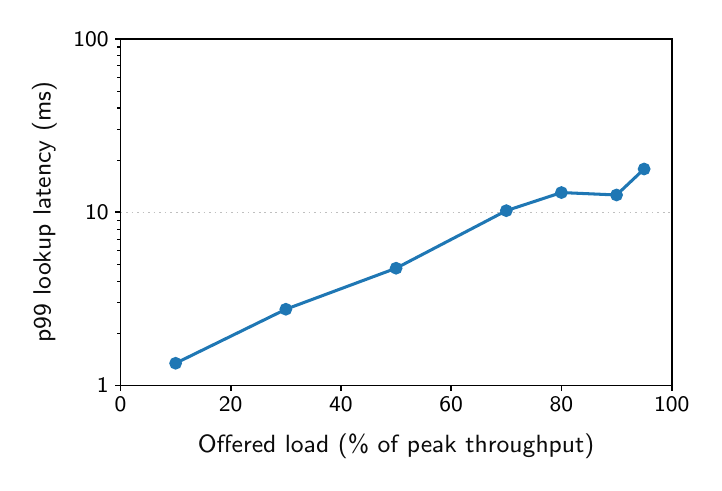
\begin{tikzpicture}[x=1cm,y=1cm]
\draw[black!25, line width=0.4pt, dash pattern=on 0.6pt off 1.4pt] (0.000,0.000) -- (7.000,0.000);
\draw[black, line width=0.6pt] (0.000,0.000) -- (-0.070,0.000);
\node[tick, anchor=east] at (-0.090,0.000) {1};
\draw[black!25, line width=0.4pt, dash pattern=on 0.6pt off 1.4pt] (0.000,2.200) -- (7.000,2.200);
\draw[black, line width=0.6pt] (0.000,2.200) -- (-0.070,2.200);
\node[tick, anchor=east] at (-0.090,2.200) {10};
\draw[black!25, line width=0.4pt, dash pattern=on 0.6pt off 1.4pt] (0.000,4.400) -- (7.000,4.400);
\draw[black, line width=0.6pt] (0.000,4.400) -- (-0.070,4.400);
\node[tick, anchor=east] at (-0.090,4.400) {100};
\draw[black, line width=0.4pt] (0.000,0.662) -- (-0.040,0.662);
\draw[black, line width=0.4pt] (0.000,1.050) -- (-0.040,1.050);
\draw[black, line width=0.4pt] (0.000,1.325) -- (-0.040,1.325);
\draw[black, line width=0.4pt] (0.000,1.538) -- (-0.040,1.538);
\draw[black, line width=0.4pt] (0.000,1.712) -- (-0.040,1.712);
\draw[black, line width=0.4pt] (0.000,1.859) -- (-0.040,1.859);
\draw[black, line width=0.4pt] (0.000,1.987) -- (-0.040,1.987);
\draw[black, line width=0.4pt] (0.000,2.099) -- (-0.040,2.099);
\draw[black, line width=0.4pt] (0.000,2.862) -- (-0.040,2.862);
\draw[black, line width=0.4pt] (0.000,3.250) -- (-0.040,3.250);
\draw[black, line width=0.4pt] (0.000,3.525) -- (-0.040,3.525);
\draw[black, line width=0.4pt] (0.000,3.738) -- (-0.040,3.738);
\draw[black, line width=0.4pt] (0.000,3.912) -- (-0.040,3.912);
\draw[black, line width=0.4pt] (0.000,4.059) -- (-0.040,4.059);
\draw[black, line width=0.4pt] (0.000,4.187) -- (-0.040,4.187);
\draw[black, line width=0.4pt] (0.000,4.299) -- (-0.040,4.299);
\draw[black, line width=0.6pt] (0.000,0.000) -- (0.000,-0.070);
\node[tick, anchor=north] at (0.000,-0.090) {0};
\draw[black, line width=0.6pt] (1.400,0.000) -- (1.400,-0.070);
\node[tick, anchor=north] at (1.400,-0.090) {20};
\draw[black, line width=0.6pt] (2.800,0.000) -- (2.800,-0.070);
\node[tick, anchor=north] at (2.800,-0.090) {40};
\draw[black, line width=0.6pt] (4.200,0.000) -- (4.200,-0.070);
\node[tick, anchor=north] at (4.200,-0.090) {60};
\draw[black, line width=0.6pt] (5.600,0.000) -- (5.600,-0.070);
\node[tick, anchor=north] at (5.600,-0.090) {80};
\draw[black, line width=0.6pt] (7.000,0.000) -- (7.000,-0.070);
\node[tick, anchor=north] at (7.000,-0.090) {100};
\draw[line width=1.1pt, line join=round, draw=cA] (0.700,0.283) -- (2.100,0.969) -- (3.500,1.490) -- (4.900,2.221) -- (5.600,2.451) -- (6.300,2.420) -- (6.650,2.750);
\filldraw[fill=cA, draw=cA, line width=0.8pt] (0.700,0.283) circle (1.9pt);
\filldraw[fill=cA, draw=cA, line width=0.8pt] (2.100,0.969) circle (1.9pt);
\filldraw[fill=cA, draw=cA, line width=0.8pt] (3.500,1.490) circle (1.9pt);
\filldraw[fill=cA, draw=cA, line width=0.8pt] (4.900,2.221) circle (1.9pt);
\filldraw[fill=cA, draw=cA, line width=0.8pt] (5.600,2.451) circle (1.9pt);
\filldraw[fill=cA, draw=cA, line width=0.8pt] (6.300,2.420) circle (1.9pt);
\filldraw[fill=cA, draw=cA, line width=0.8pt] (6.650,2.750) circle (1.9pt);
\draw[black, line width=0.6pt] (0.000,0.000) rectangle (7.000,4.400);
\node[lab, anchor=north] at (3.500,-0.550) {Offered load (\% of peak throughput)};
\node[lab, rotate=90, anchor=south] at (-0.750,2.200) {p99 lookup latency (ms)};
\end{tikzpicture}}%
\pdfvariable horigin=0pt
\pdfvariable vorigin=0pt
\pagewidth=\dimexpr\wd0+8pt\relax
\pageheight=\dimexpr\ht0+\dp0+8pt\relax
\shipout\vbox{\kern4pt\hbox{\kern4pt\box0\kern4pt}\kern4pt}
\end{document}
